\chapter{Capacitively Coupled Pixel Detectors for the CLIC Vertex Detector}
\label{chap:theory}

\chapterquote{There, sir! that is the perfection of vessels!}
{Jules Verne, 1828--1905}

\section{Introduction}
Explain why capcitivly coupled pixel detectors are a good thing and worth looking at for the CLIC vertex detectors.  Lots of good references i.e. both the HV-CMOS papers.

\section{Construction}
Description of construction information based on fabrication note.

\section{Device Characterisation}

\subsection{CLICPix Calibration}
Compare the HV-CMOS pulse height to the ToT recorded on the CLICPix using strontium 90 sources.  Gives indication of gluing layer and CLICPix capacitances.  

\begin{itemize}
\item ToT vs pulse heights.  
\item ToT vs rise times.  
\end{itemize}

\begin{figure}
\centering
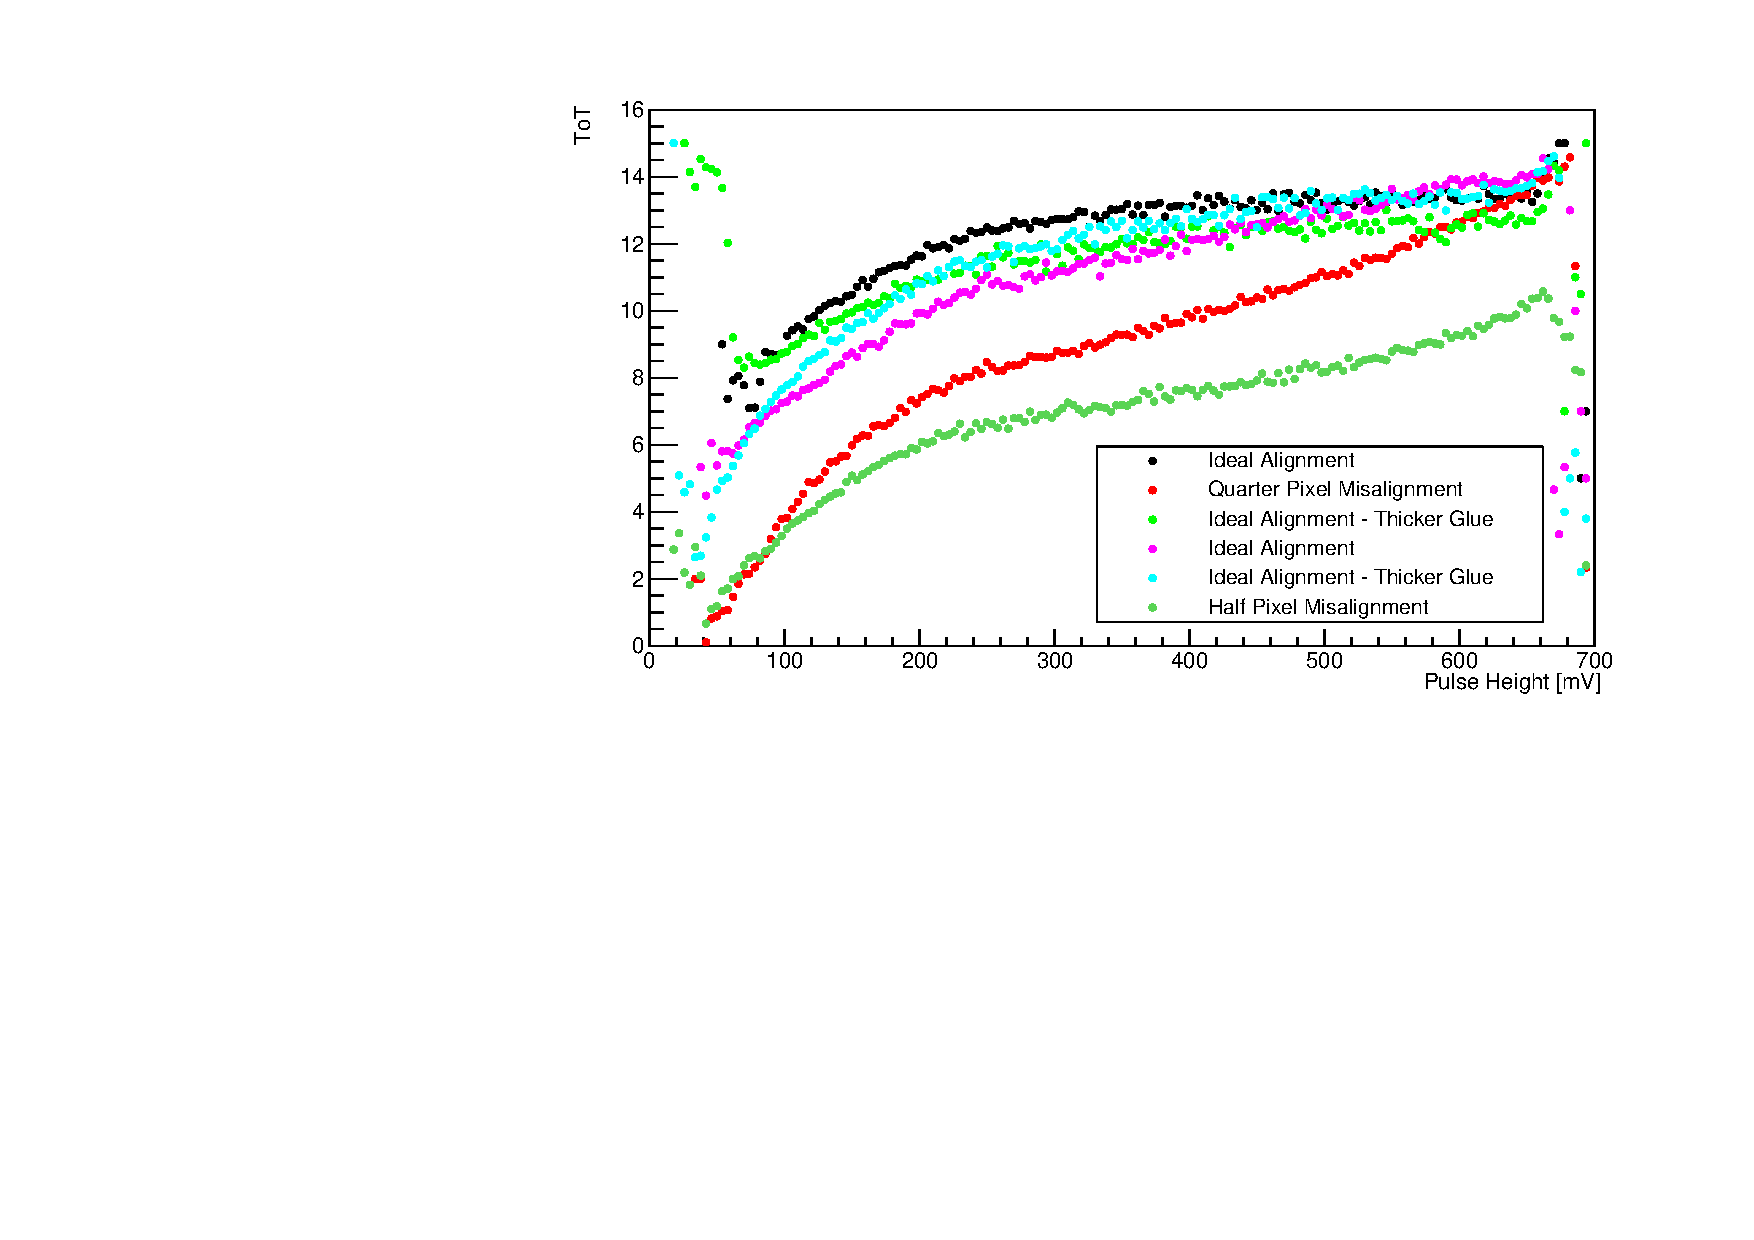
\includegraphics[width=0.5\textwidth]{CLICdpVertex/Plots/TargetToT_vs_PulseHeight.pdf}
\caption[Average ToT vs pulse height.]{Average ToT vs pulse height.}
\label{fig:avgtotvspulseheight}
\end{figure}

\begin{figure}
\centering
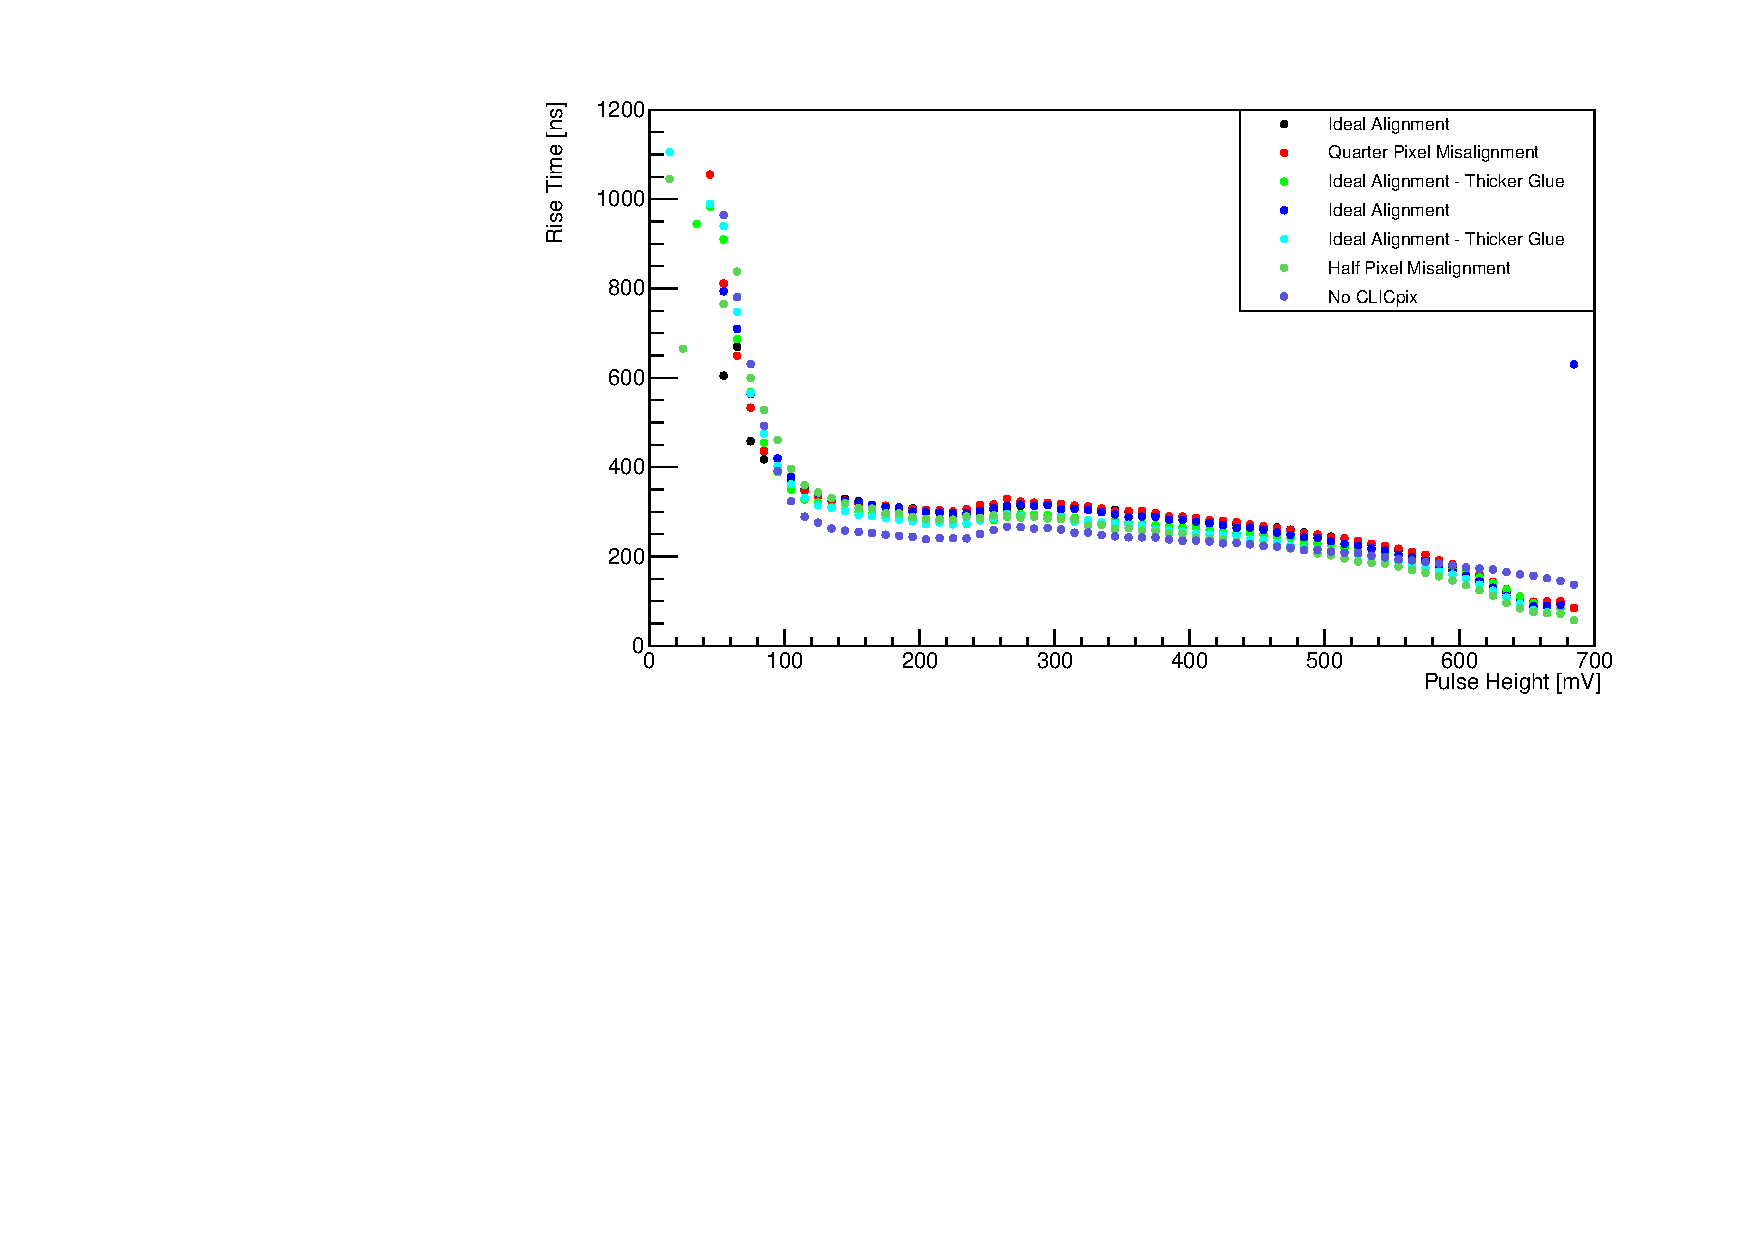
\includegraphics[width=0.5\textwidth]{CLICdpVertex/Plots/RiseTime_vs_PulseHeight.pdf}
\caption[Rise time vs pulse height.]{Rise time vs pulse height.}
\label{fig:risetimevspulseheight}
\end{figure}

\subsection{Cross Couplings}
ToT on adjacent cells vs pulse heights.  No charge sharing apparent except for SET16.  Possible issues with manufacturing other offset samples as some charge sharing is expcted.

\begin{figure}
\centering
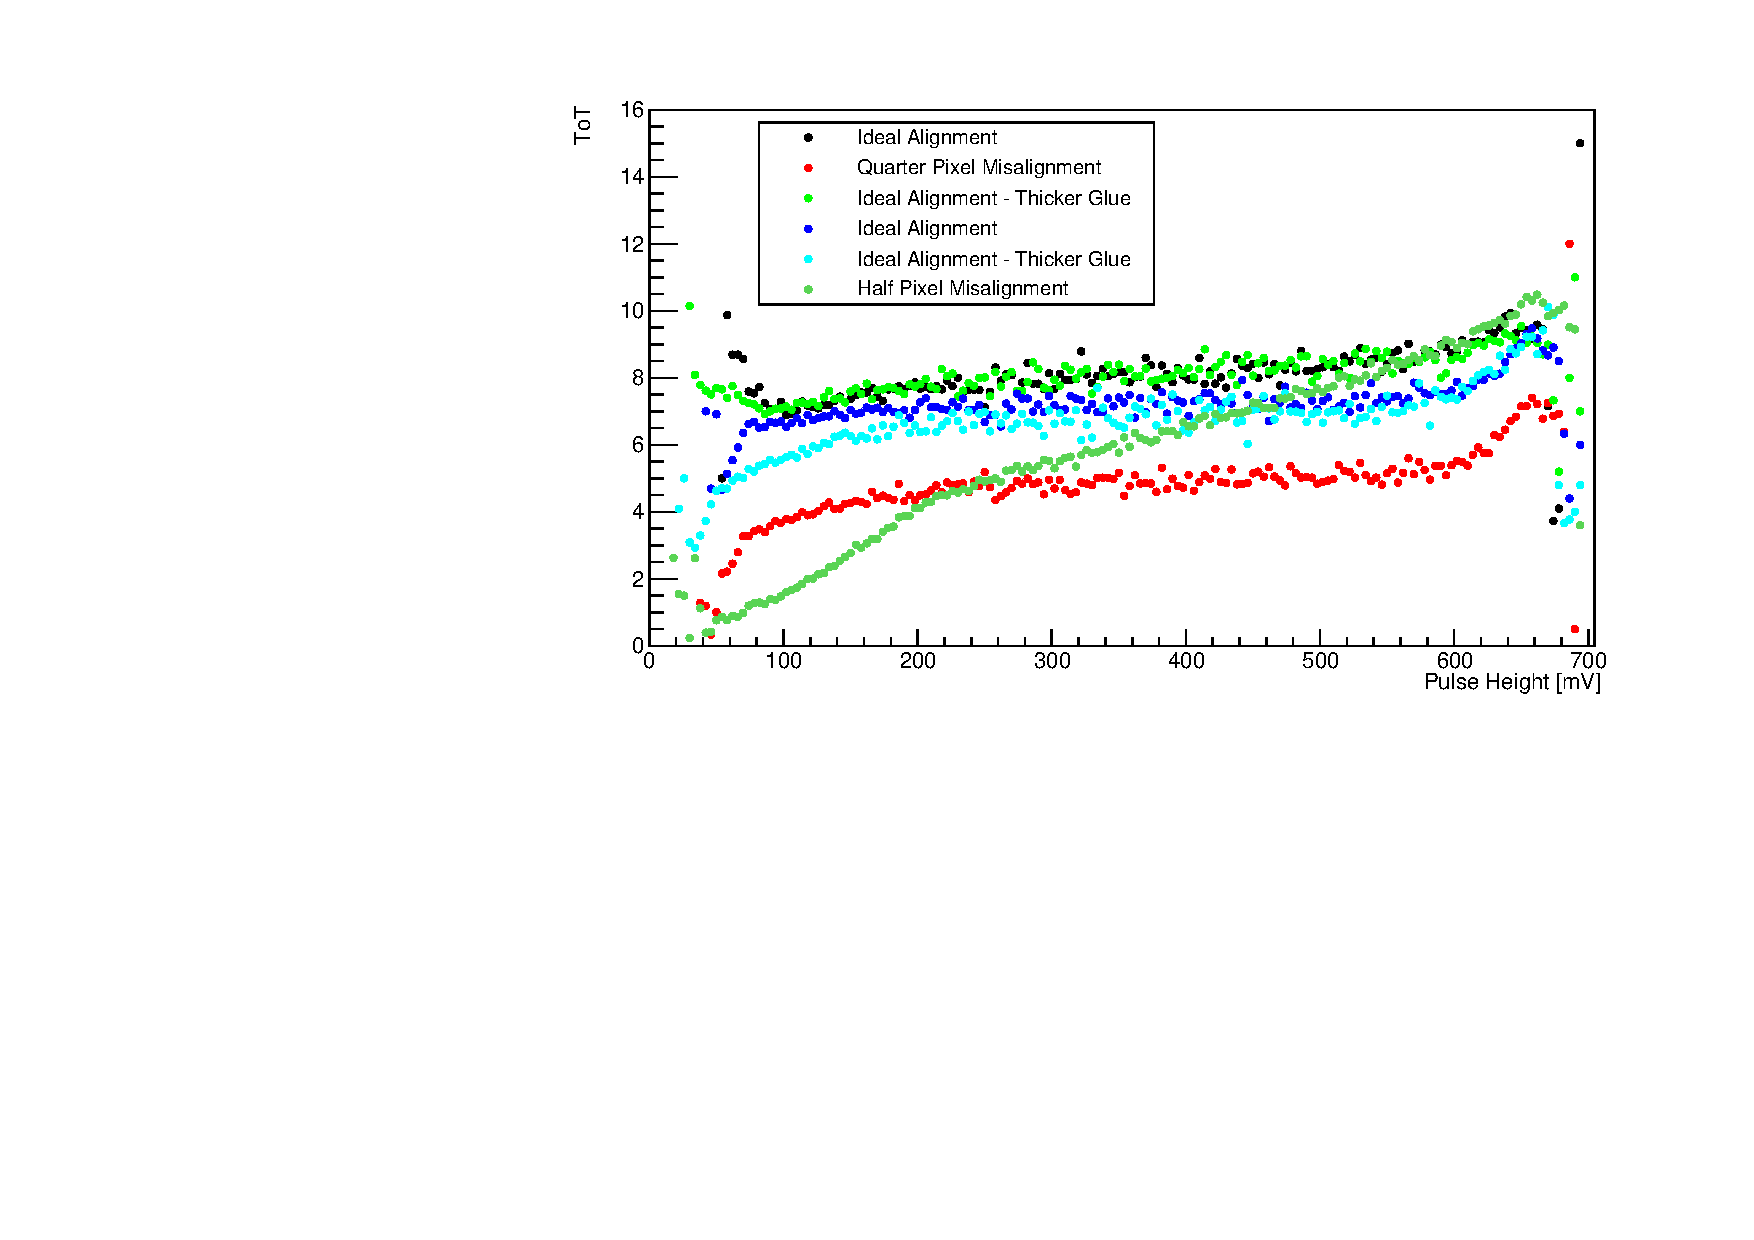
\includegraphics[width=0.5\textwidth]{CLICdpVertex/Plots/ToT_X_vs_PulseHeight.pdf}
\caption[Average ToT on adjacent pixel vs pulse height.]{Average ToT on adjacent pixel vs pulse height.}
\label{fig:avgtotadjvspulseheight}
\end{figure}

\subsection{Test Pulse Calibration}
Inject pulse height of fixed size directly into CLICPix and recored ToT.  This cannot be done for the HV-CMOS due to the device construction preventing getting to the relevant input to the HV-CMOS.  Plots of average ToT vs pulse height, describe surrogate function fit and column structure.  

\section{Test Beam Analysis}
\subsection{Test Beam Area}
Description of test beam, site and telescope.

\subsection{Efficiency}

\begin{itemize}
\item Description of masks and why they need to be applied.
\item Alignment description.
\item Efficiency calculations and conclusions. 
\end{itemize}

\begin{figure}
\centering
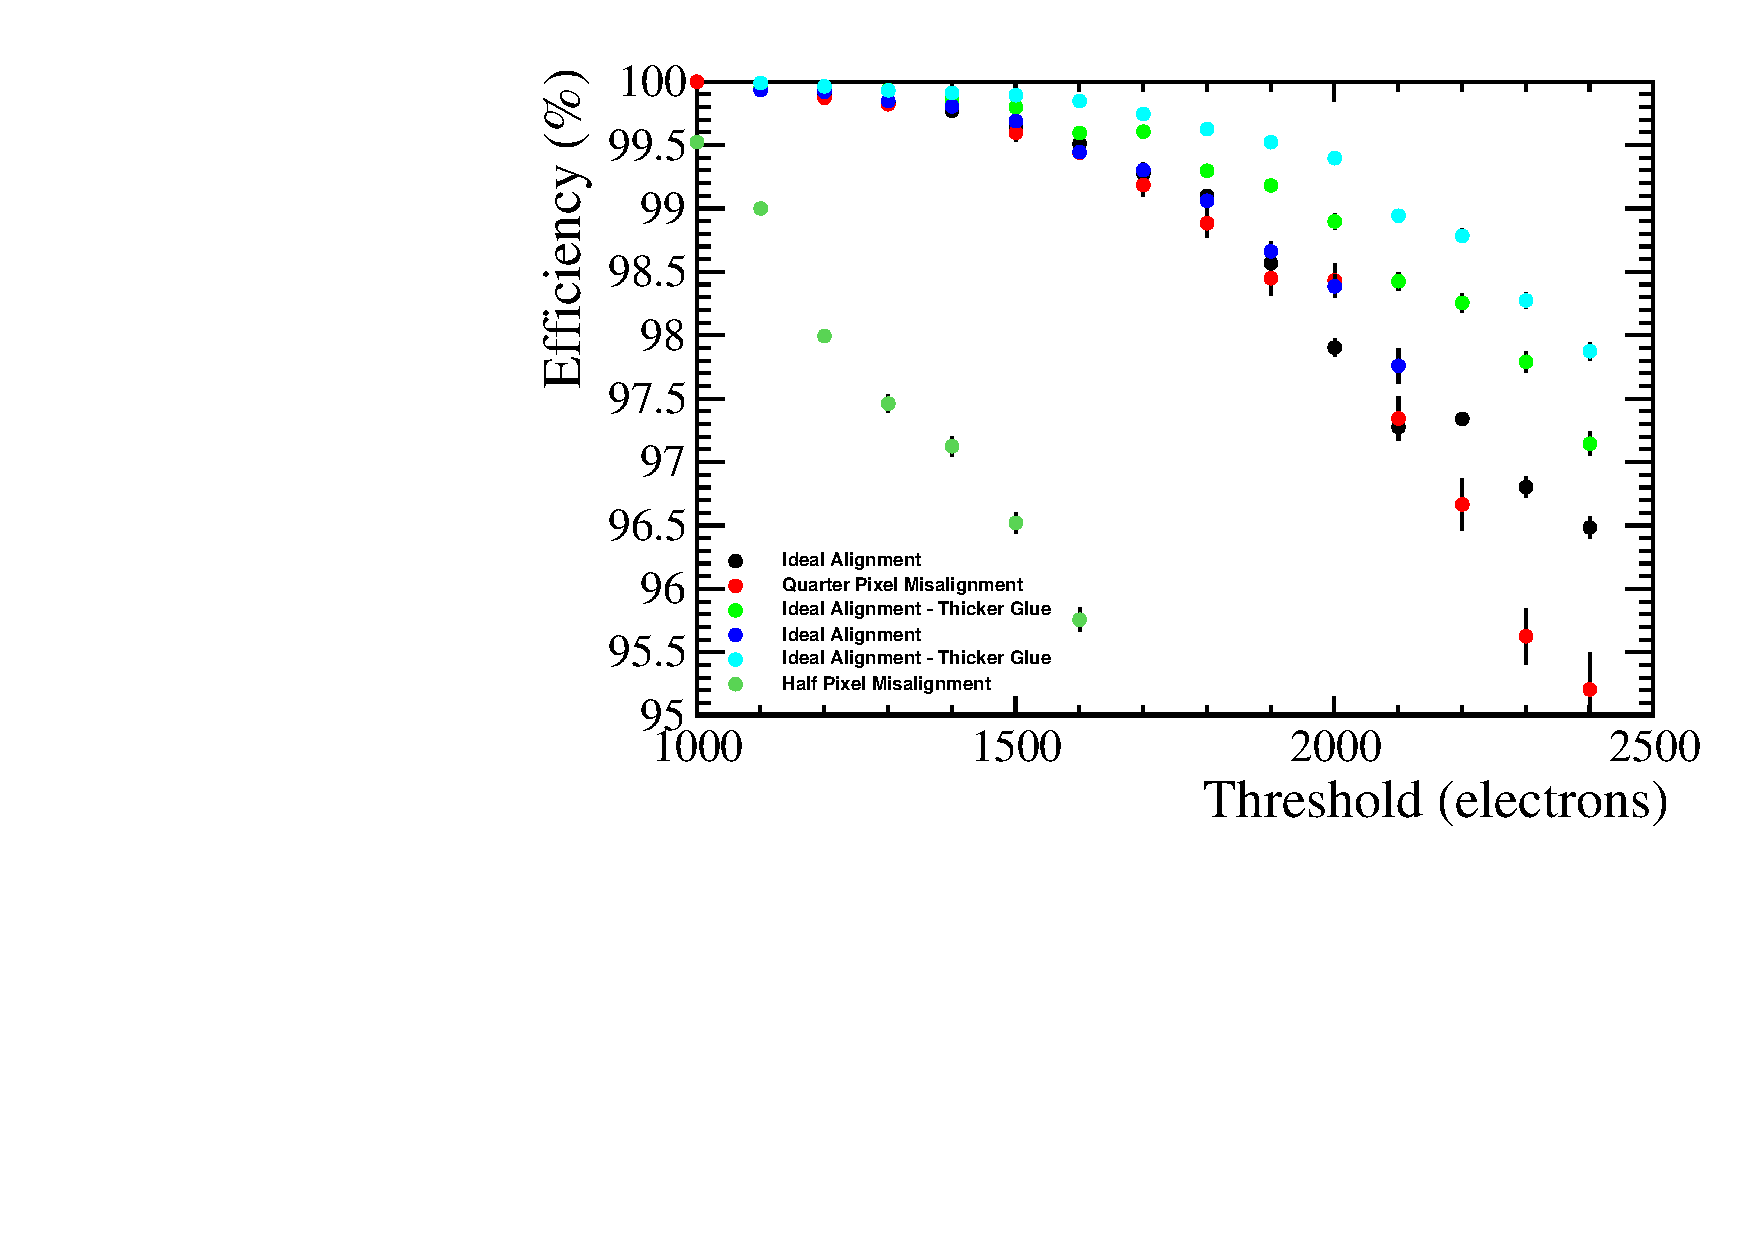
\includegraphics[width=0.5\textwidth]{CLICdpVertex/Plots/ZoomedEfficiency.pdf}
\caption[Efficiency vs threshold.]{Efficiency vs threshold.}
\label{fig:efficiency}
\end{figure}




  
